\graphicspath{ {Implementation/Images/} }


\chapter{Validation}
\label{cha:implementation}

\section{Introduction}
In this chapter 

DiseaseMapping (generalization)
OSIM
Clusters
TensorFlow
DL4J

MENTION THAT LSTM CAN ALSO BE USED TO VALIDATE AND IS A BETTER WAY TO VALIDATE THIS METHOD


\section{Dataset}

To validate the approaches mentioned in chapter \ref{cha:background}, we used a dataset generated by OSIM2. This dataset is used by OMOP to validate their methods to predict the effects of drug treatments. It contains around $10$ million of hypothetical patients based on Thomson Reuters MarketScan Lab Database (MSLR). MSLR contains administrative claims between 2003 ad 2009 from a privately-insured population. \\

The OSIM2 dataset is contains multiple database tables which are dumped as comma-separated values (csv) files. To make it easier to work with this dataset, we joined the multiple files into one file with on each row an event of a patient containing all relevant information. The relevant information which is kept is: birth year, gender, condition type, condition, time difference since previous diagnosis, and season (summer, fall, winter, spring). Thus, one EHR is $7$ dimensional. \\	

Using our approaches on this dataset, we can compare our results to the found clusters in Anders Boeck Jensen et. \cite{Brunak:article}. Although these found clusters are not a golden standard, it is a first validation point for our approaches.


\section{Software}

\subsection{TensorFlow}

TensorFlow is an open-source machine learning software library released at the end of 2015 \cite{tensorflow:article}. It is developed by the Google Brain Team. \\
It provides a Python interface for efficient C++ code. After some time, we found that Tensorflow is not well documented at the moment and does not gave the needed freedom to easily rewrite some core features of their Word2Vec implementation, for example manipulating the internal trained lookup table.


\subsection{DeepLearning4Java}

DeepLearning4Java (DL4J) is an open-source machine learning software library released by Skymind \cite{dl4j:article}. \\
It runs on their scientific computing engine ND4J which provides fast matrix operations. DL4J is completely written in Java and provides a lot of freedom to manipulate lookup tables and extend their Word2Vec methods to work on abstract object like vectors. The developers are active on Gitter and offer a lot of information on how to use certain parts of DL4J. 


\section{Experiment Setup}

\subsection{Generalization}

As described in chapter \ref{cha:background}, we use generalized Word2Vec approaches to find patterns in EHR data. We use the OSIM dataset and represent each EHR as a $7$ dimensional vector. This vector is comparable to a word in a normal Word2Vec approach and functions as the abstract object in our generalized Word2Vec approaches. \\

Because we are working with high dimensional data, most instances of OMOP are quite unique. This is mainly due to a combination of specific disease codes and time intervals. To find patterns which are more general applicable, we start with generalizing our data. With generalizing we mean that values for some attributes are projected into categories. For example, the time intervals are projected into $4$ categories. \\

It is easy to generalize concepts as time intervals and demographics, for example we can say that people between the age $0$ and $10$ belong to category A. This becomes complex for disease diagnoses as it is domain specific and requires a lot of knowledge to generalize those. We talk about our solution to this in section \ref{sec:mapping}. \\

To see the effect of our generalization, see table \ref{tab:general}. You can see the $3$ most common vectors from our dataset before and after the generalization. \\

\begin{table}[]
\centering

\label{tab:general}
\begin{tabular}{ll}
\cline{1-1}
\multicolumn{1}{|l|}{\textbf{Before Generalization}}                     & {\ul }                                   \\ \hline
\multicolumn{1}{|l|}{\textit{Vector}}                                    & \multicolumn{1}{l|}{\textit{Occurences}} \\ \hline
\multicolumn{1}{|l|}{{[}1956.0, 8532.0, 65.0, 5.00000701E8, 0.0, 3.0{]}} & \multicolumn{1}{l|}{17574}               \\ \hline
\multicolumn{1}{|l|}{{[}1954.0, 8532.0, 65.0, 5.00000701E8, 0.0, 3.0{]}} & \multicolumn{1}{l|}{17536}               \\ \hline
\multicolumn{1}{|l|}{{[}1955.0, 8532.0, 65.0, 5.00000701E8, 0.0, 3.0{]}} & \multicolumn{1}{l|}{17476}               \\ \hline
                                                                         &                                          \\ \cline{1-1}
\multicolumn{1}{|l|}{\textbf{After Generalization}}                      &                                          \\ \hline
\multicolumn{1}{|l|}{\textit{Vector}}                                    & \multicolumn{1}{l|}{\textit{Occurences}} \\ \hline
\multicolumn{1}{|l|}{{[}6.0, 8532.0, 65.0, 784955.0, 1.0, 3.0{]}}        & \multicolumn{1}{l|}{282086}              \\ \hline
\multicolumn{1}{|l|}{{[}7.0, 8532.0, 65.0, 784955.0, 1.0, 3.0{]}}        & \multicolumn{1}{l|}{235459}              \\ \hline
\multicolumn{1}{|l|}{{[}5.0, 8532.0, 65.0, 784955.0, 1.0, 3.0{]}}        & \multicolumn{1}{l|}{230216}              \\ \hline
\end{tabular}

\caption{Three most common vectors in our dataset before and after generalization}
\end{table}


\subsection{Disease Code Mapping}
\label{sec:mapping}

In the section we discuss the method to generalize the disease codes used to label the diagnoses in the OMOP dataset. The basic idea is that we want to generalize the diagnoses. For example, a bruise on your right leg is the same diagnoses as a bruise on your left leg. \\

The OMOP dataset uses MedDRA disease codes for the diagnoses. We described the MedDRA disease codes in chapter \ref{cha:context}. We mentioned that MedDRA does not have a clear hierarchy. With a clear hierarchy, it would be trivial to generalize a disease code to its highest hierarchy. \\
To solve this, we map the MedDRA disease codes to the ICD 10 disease codes. The reason behind this is that ICD 10 provides a clear and easy to use hierarchy. Besides the easy to use hierarchy, we also need the ICD 10 disease codes to make it possible to compare our results with Anders Boeck Jensen et. \cite{Brunak:article} as their results also use ICD 10 disease codes. \\

The mapping is based on the description of each disease code. Both MedDRA and ICD 10 have a short medical description of each code. Each description is first filtered from stop words. Afterwards, the MedDRA code is matched to the ICD 10 code based on the matching of both description. The matching is done on the highest percentage of words matching. \\

In figure \ref{fig:mappingStats}, we show the statistics of this mapping process. Note that we only take disease codes into account if they are also part of the OMOP dataset. In the figure, each bar represents the percentage of the words matching between descriptions. The height of the bars represent the percentage of all disease codes in the OMOP dataset who have this amount of matching percentage.

\begin{figure}[H]
	\centering
	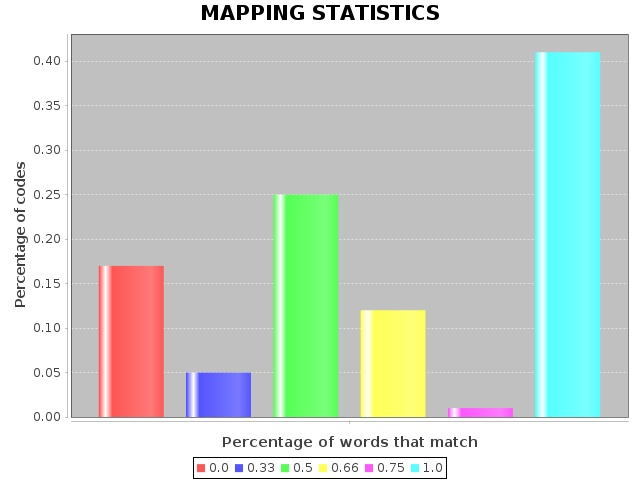
\includegraphics[width=0.7\textwidth]{mappingStats.jpeg}
	\caption{Statistics of the mapping approach}
	\label{fig:mappingStats}
\end{figure}

We have an average of $63$ \% of the words from the description that matches between MedDRA and ICD 10 descriptions. We also see that around $85$ \% of all the disease code mappings have a match of atleast $33$ \%. We assume this is already a good mapping as medical terms are quite specific and if $33$ \% matches, the upper hierarchy will be a good enough match. For the codes which have a zero percent match, the Damerau-Levenshtein algorithm \cite{edit:article} is applied. The algorithm calculates the edit distance between two strings using character insertion, character deletion, character replacement, and adjacent character swaps. The description with the lowest edit distance, is then chosen as best match.

\section{Results}
-what to test

\section{Conclusion}


http://omop.org/OSIM2


%%% Local Variables: 
%%% mode: latex
%%% TeX-master: "thesis"
%%% End: 
